%%%%%%%%%%%%%%%%%%%%%%%%%%%%%%%%%%%%%%%%%
% Short Three-Column Newsletter
% LaTeX Template
% Version 1.0 (11/9/13)
%
% Original author:
% Frits Wenneker (http://www.howtotex.com) 
% With extensive modifications by:
% Vel (vel@latextemplates.com)
% 
% This template has been downloaded from:
% http://www.LaTeXTemplates.com
%
% License:
% CC BY-NC-SA 3.0 (http://creativecommons.org/licenses/by-nc-sa/3.0/)
%
%%%%%%%%%%%%%%%%%%%%%%%%%%%%%%%%%%%%%%%%%

%----------------------------------------------------------------------------------------
%	PACKAGES AND DOCUMENT CONFIGURATIONS
%----------------------------------------------------------------------------------------

\documentclass[10pt,a4paper]{article} % Paper type (a4paper, usletter or legal) and font size (10, 11 or 12)

\setlength\topmargin{-48pt} % Top margin
\setlength\headheight{0pt} % Header height
\setlength\textwidth{7.0in} % Text width
\setlength\textheight{9.5in} % Text height
\setlength\oddsidemargin{-30pt} % Left margin
\setlength\evensidemargin{-30pt} % Left margin (even pages) - only relevant with 'twoside' article option

\usepackage{charter} % Charter font for main content
\usepackage{siunitx}
\frenchspacing % Reduces space after periods to make text more compact for a three-column layout

\usepackage{graphicx} % Required for including images
\usepackage{amssymb,amsmath} % Math packages
\usepackage{multicol} % Required for the three-column layout of the document
\usepackage{url} % Clickable links
\usepackage{enumitem} % Reduces the amount of space within and between lists with [noitemsep,nolistsep]
\usepackage{marvosym} % Required for the use of symbols
\usepackage{wrapfig} % Allows wrapping text around figures
\usepackage[T1]{fontenc} % Use 8-bit encoding that has 256 glyphs
\usepackage{datetime} % Required for defining a custom date style
\newdateformat{mydate}{\monthname[\THEMONTH] \THEYEAR} % Set a custom date format
\usepackage[pdfpagemode=FullScreen, colorlinks=false]{hyperref} % Link colors and PDF behavior in Acrobat
\usepackage{fancyhdr} % Required to define custom headers/footers
\pagestyle{fancy} % Enables the custom headers/footers for all pages following this

%-----------------------------------------------------------
% Header and footer
\lfoot{\footnotesize % Left footer containing newsletter contact information
	Greek islands, a paradise on earth\\
	\Mundus\ \href{https://github.com/stefanos1316/my_blog/index.com}{my\_blog/index.com} \quad
	%\Telefon\ Not available yet \quad
	\Letter\ \href{mailto:sgeorgiou@aueb.gr}{sgeorgiou@aueb.gr}
}


\cfoot{} % Empty center footer

\rfoot{\footnotesize ~\\ Page \thepage} % Right footer - page counter

\renewcommand{\headrulewidth}{0.0pt} % No horizontal rule for the header
\renewcommand{\footrulewidth}{0.4pt} % Horizontal rule separating the footer from the document
%-----------------------------------------------------------

%-----------------------------------------------------------
% Define separators
\newcommand{\HorRule}[1]{\noindent\rule{\linewidth}{#1}} % Creates a horizontal rule
\newcommand{\SepRule}{\noindent	% Creates a shorter separator rule
\begin{center}
\rule{250pt}{1pt} % Page width and rule width
\end{center}
}
%-----------------------------------------------------------

%-----------------------------------------------------------
% Define title and article styles
\newcommand{\NewsletterName}[1]{ % Newsletter title
\begin{center}
\Huge \usefont{T1}{fvs}{b}{n} % Use the Bera Sans Bold font
#1
\end{center}	
\par \normalsize \normalfont}

\newcommand{\JournalIssue}[1]{ % Date and issue number at the top of the newsletter
\hfill \textsc{\mydate \today, No #1} % Right-aligned date and issue number
\par \normalsize \normalfont}

\newcommand{\NewsItem}[1]{ % News item title
\usefont{T1}{fvs}{n}{n} % Use the Bera Sans Normal font
\vspace{24pt}\large #1\vspace{3pt} % Print the title with space around it in a larger font size
\par \normalsize \normalfont}

\newcommand{\NewsAuthor}[1]{ % Author name under the item title
\hfill by \textsc{#1} \vspace{20pt} % Right-aligned author name in small caps with space after it
\par \normalfont}		

%----------------------------------------------------------------------------------------
%	TITLE
%----------------------------------------------------------------------------------------

\begin{document}

\JournalIssue{1} % Issue number

\NewsletterName{Visiting the paradise islands} % Newsletter title

\noindent\HorRule{3pt} \\[-0.75\baselineskip] % Thick horizontal rule
\HorRule{1pt} % Thin horizontal rule

%----------------------------------------------------------------------------------------
%	MAIN NEWS ITEM
%----------------------------------------------------------------------------------------

\vspace{0.5cm}
\SepRule
\vspace{-0.5cm}

\begin{center}
\begin{minipage}[h]{0.84\linewidth}
\begin{wrapfigure}{l}{0.44\textwidth}
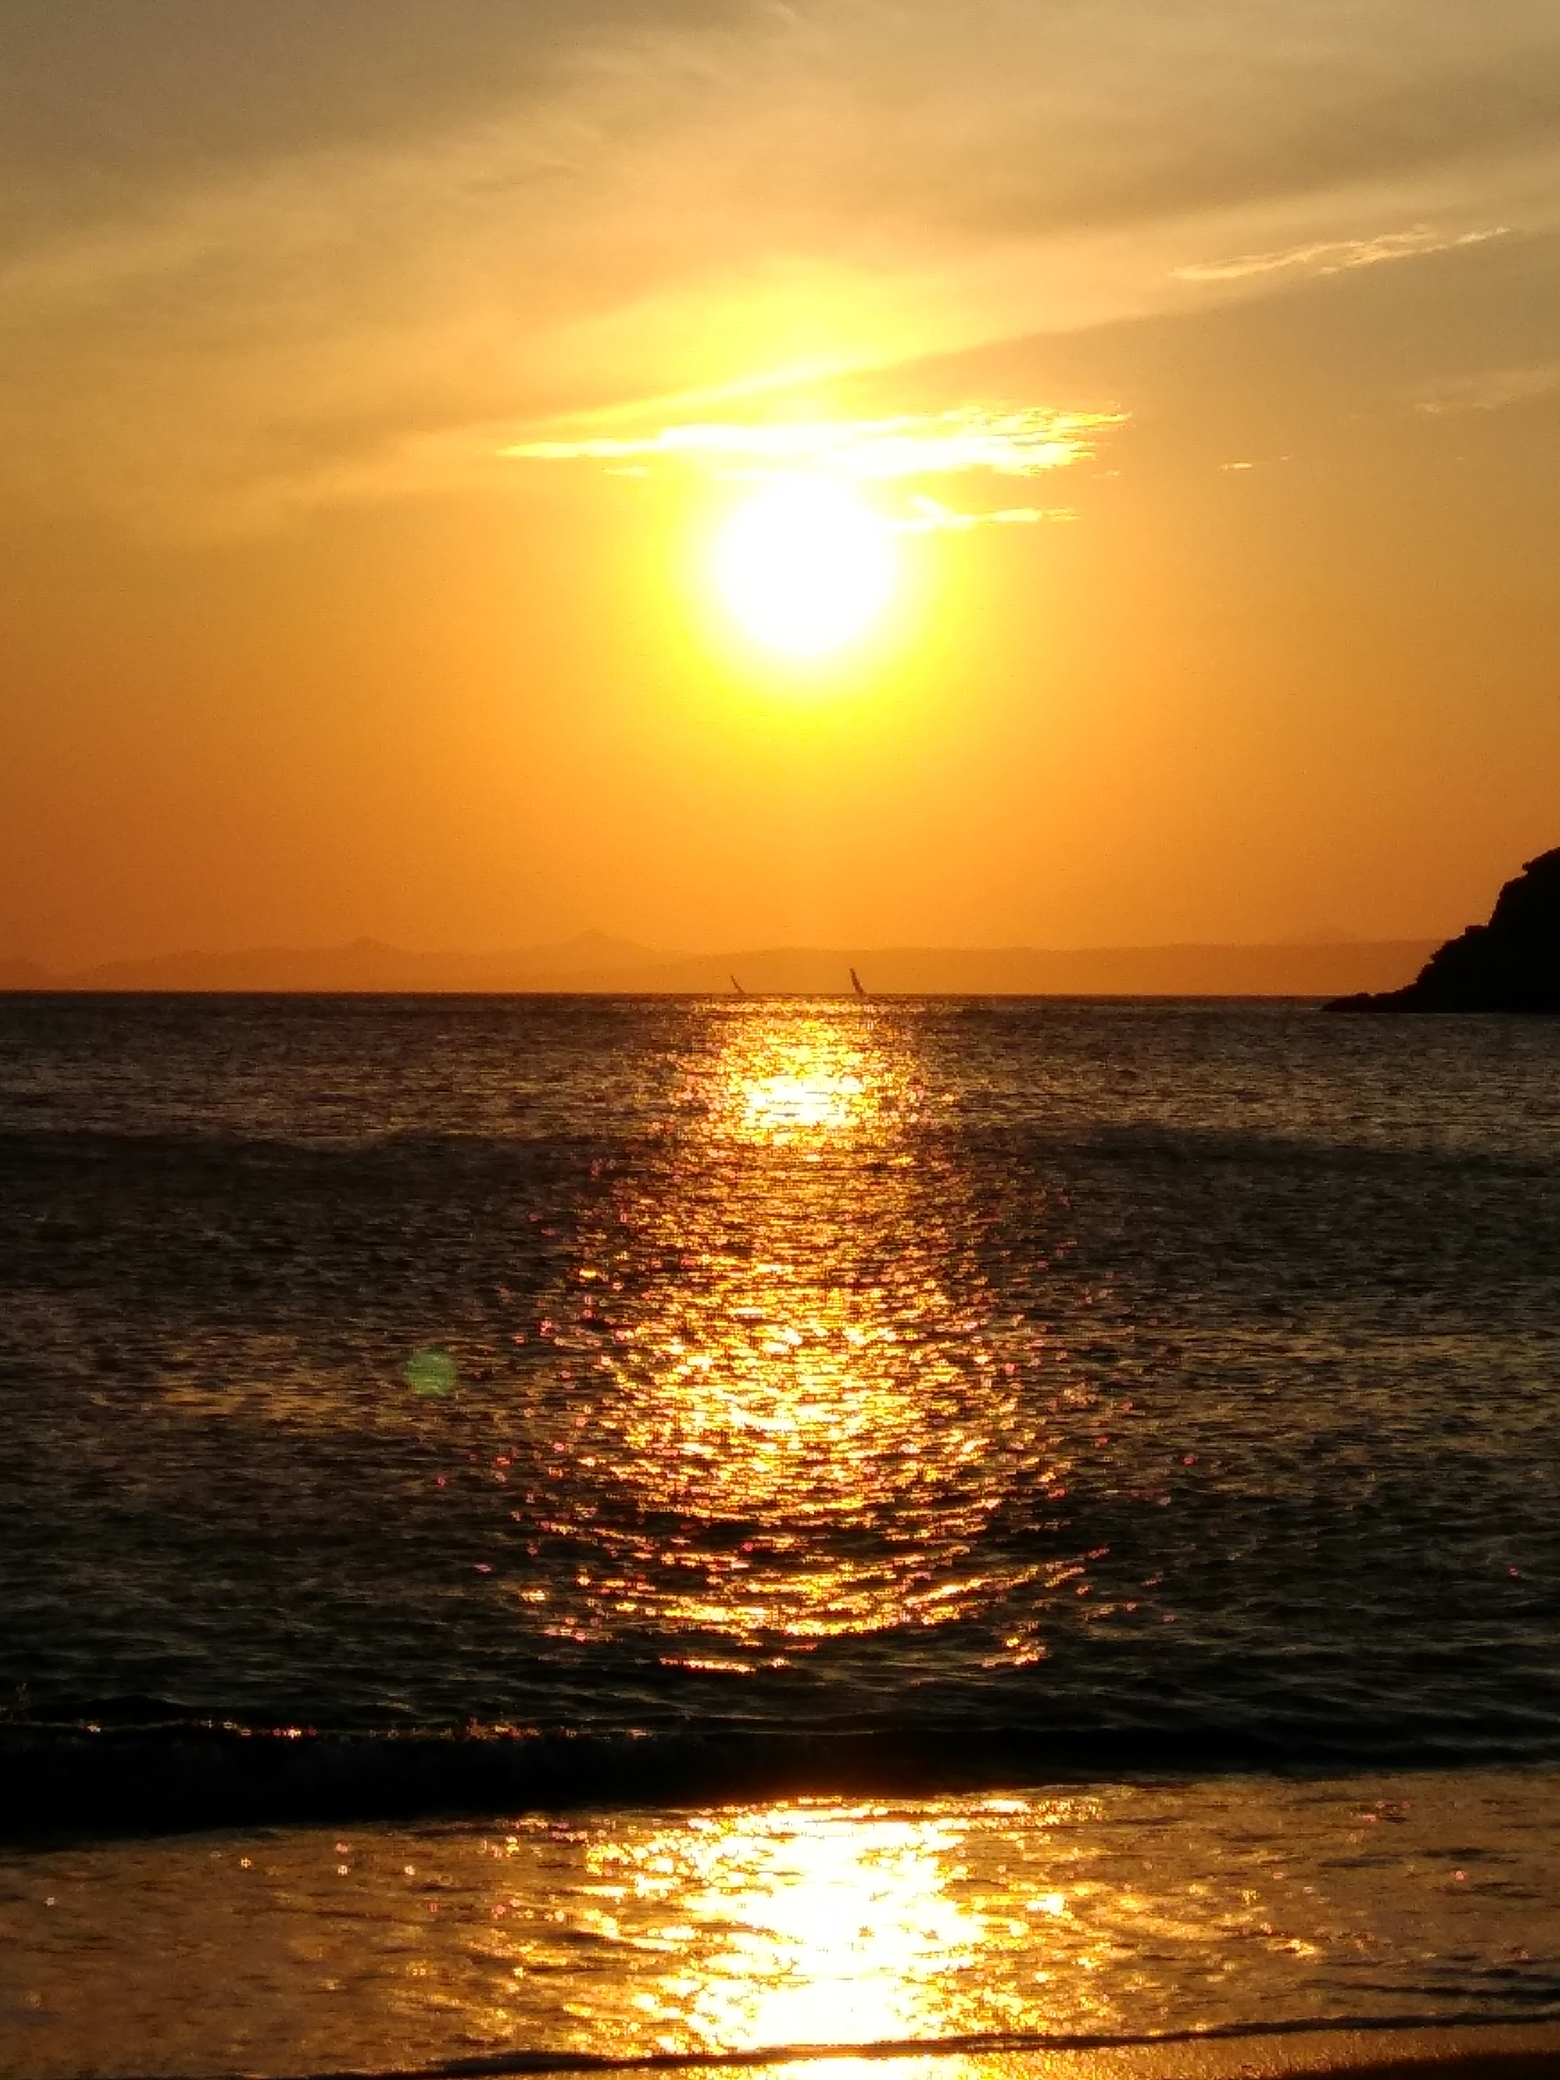
\includegraphics[width=0.4 \textwidth]{media/front_picture.jpg}
\\
\end{wrapfigure}
	
\NewsItem{Author's thoughts} % Main next item title
\vspace{3pt} % Some extra whitespace since there is no author as for the news in the body of the newsletter
\textit{
%12345678901234567890123456789012345678901234567890123456789012345678901234567890
Greece, the country of democracy, a place where great philosophers were born, 
culture and art was produced, but also a country that does not lack of 
environmental beauty. 
This charm of Greece, in my believe, lies in the vast set of small islands which offer 
simplicity, relaxation, and endless moments of happiness. 
The bizarre feeling when landing on an island, a new place to discover, a 
different adventure to experience is all about what Greek islands offer to their 
visitors.
Before start pursuing my Doctorate degree, in Athens, I have never visited any 
Greek island before. 
However, after starting visiting them my jaws dropped every time. 
A feeling of enthusiasm covers my mind of each islands unique character, 
their different way of living, and the openness of their locals.
Many times, I catch my self saying the same thing, ``when I become pensioner I am 
going to by a small house in a Greek island and living a chill, quiet, and easy 
going live...''
}
\par\hfill --- Stefanos Georgiou
\end{minipage}
\end{center}

\vspace{0.5cm}
\SepRule % Small horizontal rule after the main news item
\vspace{0.5cm}

%\setlength{\columnsep}{16pt} % Uncomment to manually change the white space between columns
\begin{multicols}{3} % Begin the three-column layout

%----------------------------------------------------------------------------------------
%	OTHER NEWS
%----------------------------------------------------------------------------------------

\NewsItem{A visit in Haven}
\NewsAuthor{Stefanos Georgiou}

%12345678901234567890123456789012345678901234567890123456789012345678901234567890
In 2010, Greece was officially announced as a country of economic crisis, 
a fact that goes on over eight years, nowadays. 
However, a part that Greece is never on crisis is the unimaginable beauty and charm 
of its environment and more specifically its islands. 
The combination of sunny weather, almost all year along, with the exceptionally 
large and tasty portions of food, the great hospitality of its people, and the 
intense night live are the reasons making many tourists daydreaming when they talk 
about Greece all over the world.  


%12345678901234567890123456789012345678901234567890123456789012345678901234567890
According to Wikipedia, Greece has around 1,200 to 1,600 islands where 227 
are inhabited. 
It also offers, beaches with various sandy colours such as brown, white, golden, 
pink, and volcanic black. 
In addition, it is a country with the most blue flagged beaches in Europe that 
indicates the clean waters. 
Tourists can enjoy their stay in islands by stay in hotels, apartments, or even 
camping sites which various of them do exist. 
However, my suggestion is not to stay for long time at hotel resorts, but, instead 
travel to different villages, talk with locals, go the places that also locals 
go in order to learn from this culture.  


%12345678901234567890123456789012345678901234567890123456789012345678901234567890
During my accommodation in Greece, I was fortune to visit at least ten different 
islands from various seas. 
Greece's islands can be found both in Aegean and Ionian seas. 
The distinguished characteristics of Aegean islands is the dry climate and 
environment, but, warm seas. 
On the contrast, Ionian islands are less dry with rich environment and many 
trees, but, with much colder waters, in general. 
\textbf{Here discuss on the different complexes of islands such Cuclades, ...}
I have visited islands in both seas but mainly from the Aegean sea. 
Therefore the most of the discussion is going to be for the Aegean islands. 


%12345678901234567890123456789012345678901234567890123456789012345678901234567890
My aim with this article is to expose the hidden magic of the islands through 
some of my adventures, feelings, historical events, and thoughts in order to encourage people that 
paradise is not far away, it is much more closer than most of them think. 
  

%----------------------------------------------------------------------------------------
\NewsItem{Aigina, my first island}

%12345678901234567890123456789012345678901234567890123456789012345678901234567890
By the end of April 2016, when the temperature usually is much higher than \ang{30}, 
a friend of mine, that we used to server in army for our mandatory duty, gave me 
an unexpected call. 
He was visiting Athens with his girlfriend for few days and he wanted to travel to 
Aigina and to catch up with me.
A relatively big islands that is located at Sarronic bay and less than an hour 
distance away from Pireaus port by boat and famous mostly for the Aigina's peanuts; 
which is actually...a kind of pistachio. 


%12345678901234567890123456789012345678901234567890123456789012345678901234567890
Until that time, I have never been before to any island nor on a boat and since 
I am always up for trying new a different things I took the call. 
In general, in low season, there is no need to pre-book boat tickets since not 
many people are visiting the islands. 
After we bought our tickets, we entered the boat and took a place outside where 
to have better view and stair the seagulls. 
The seagulls were flying most of the time next to the boat to fish. 
Many people were trying to feed them in order to take pictures with them. 
It is necessary to be careful since the seagulls can bite also your hand while 
trying to get the food out of it. 
Therefore, we enjoy the view until we reached our destination, the port of Aigina. 


\begin{center}
	\includegraphics[width=0.32\textwidth]{media/aigina_2.jpg}
	\par\textit{Aigina's port and clean waters}
\end{center}


%12345678901234567890123456789012345678901234567890123456789012345678901234567890
The port of Aigina, where we disembarked, is located in the main city. 
Each island of Greece has its own main city and in most case a port can also be 
found there. 
In the old times, for some islands, the locals were building their main cities 
on mountains away from the port. 
This was done since to avoid quick attacks from pirates. 
However, it was not the case for Aigina. 


\begin{center}
	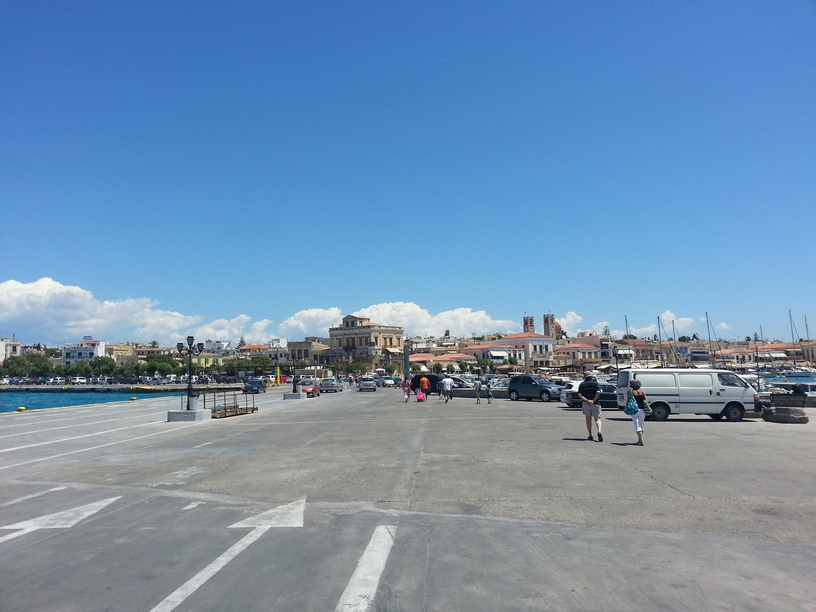
\includegraphics[width=0.32\textwidth]{media/aigina_1.jpg}
	\par\textit{Aigina's main city}
\end{center}


%12345678901234567890123456789012345678901234567890123456789012345678901234567890
Once we disembarked, we took a ride towards Marathonas beach since it is found 
outside of the city and the bus schedules are not in favour of the public. 
However, on my second tour to Aigina I was more prepared and I rented a bike which 
was much fun and a cheaper solution.
The organised beaches in Greece offer umbrellas, beach beds, and bars from where 
you can enjoy ice-cold coffees such as frappe, cold beers, and different snacks. 
Even tho it was May and the outside temperature more that \ang{35} the water was 
quite cold for my Cypriot standards. 
Nevertheless, it was also refreshing and my first bath, so I tried to enjoy it 
as much as I could without showing that it was cold. 


%12345678901234567890123456789012345678901234567890123456789012345678901234567890
After our cold experience on Marathonas beach, we made our way back to the city 
where we enjoyed some local food and Aigina's peanuts. 
Also, we took our time to explore the city centre that provides different types of 
restaurants, mainly we Greek cuisine,  and small narrow roads where decorated with 
many bougainvillea, white house, and very clean streets. 
Just walking in those streets of Aigina you can get the feeling that some things 
in that island remained unaffected by the past of time. 
But still, the beauty and their simplicity can rest the humans soul. 
After our walk we took the boat to return to the noisy Athens once again.


%----------------------------------------------------------------------------------------
\NewsItem{Salamina}

%12345678901234567890123456789012345678901234567890123456789012345678901234567890
A place where one of the biggest naval battle between the Greece and the Persian 
army took place. 
On that time, Greece was separated in different kingdoms. 
Therefore, they united their forces to take down their common enemy. 
Also, there is a large naval base at Salamina that is hosting multiple types of 
warships.


%12345678901234567890123456789012345678901234567890123456789012345678901234567890
By the begging of May 2016, one of our lab's PhD fellow, Maria Kechagia, invited 
the whole lab in her hometown, which is in Salamina for a day trip. 
Salamina, is an island that is almost 15 minutes away by ferry boat. 
Therefore, we took the opportunity and we loaded two cars in the ferry to make our 
way easier in Salamina. 
The different between the ferry and the normal boat is that the ferry is much 
smaller and slower. 
That means strong waves and long distances are troublesome.


\begin{center}
	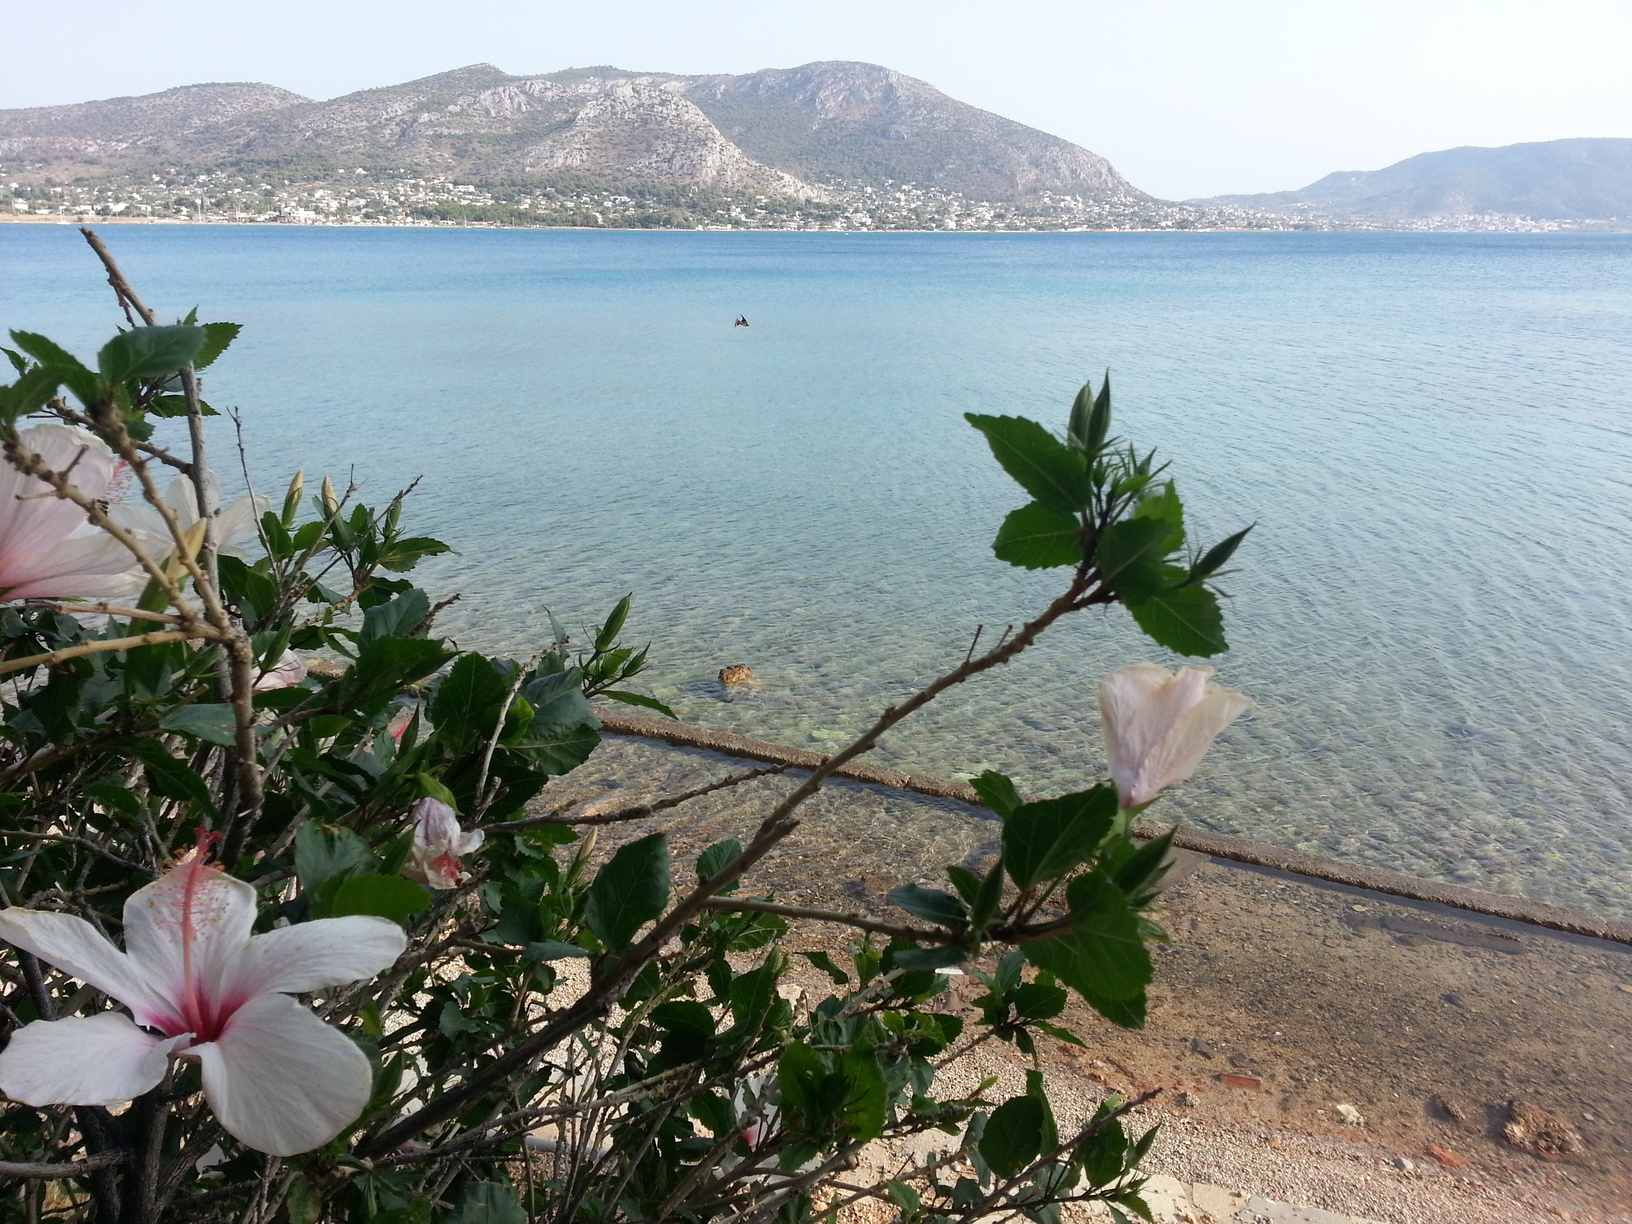
\includegraphics[width=0.32\textwidth]{media/salamina_1.jpg}
	\par\textit{The island of Salamina}
\end{center}


%12345678901234567890123456789012345678901234567890123456789012345678901234567890
Our first stop in Salamina was at Maria's home where her parents were expecting us. 
Her mother, few months ago had to go through a surgery and blood was required for 
that. 
Upon request, I immediately went for blood donation, a fact that her mother remembers 
till today and every time we meet she is bringing me cookies and other kind of sweets. 
In our company, we also had a PhD student from India who came with his wife and 
four years old kid. 
Greek parents are going crazy when they see kids and they try to cheer them with 
every kind of sweet of toys they have, no matter from which country they are. 
However, they did not only treat the kid well but us also. 
Once we sit outside in their garden that was full of trees, plants and flowers, 
Maria's mother brought us coffee, cookies, and home made ice-cream. 
Afterwards, they also suggested us beaches to visit and places to eat lunch.


%12345678901234567890123456789012345678901234567890123456789012345678901234567890
After the beach we went to have lunch at a local restaurant where we order ``kotsi''. 
This food is part of the pork's leg, cooked in an oven with sauce and different 
species. 
Literally the meat was going off the bone by simple touching it. 
It was one of the most amazing ``kotsi'' we ever had. 
Even after two years, our PhD fellow Antonis Gkortzis is still mentioning that food.     


%----------------------------------------------------------------------------------------
\NewsItem{Vacations in Milos}

%12345678901234567890123456789012345678901234567890123456789012345678901234567890
Summer in Athens is almost unbearable and an escape plan is go to a Greek island. 
Ana, a beautiful blond Slovenian girl with charming blue eyes 
and a crystal smile, came to visit me in order to go at Milos island. 
Milos is an island in Cyclades before Santorini, however, much more 
cheaper, with less tourists, and beautify sandy beaches. 
In addition, most of the Cyclades islands share the common characteristics as 
white houses, flat roofs, blue doors and window labels, in most of cases. 
Therefore, in mid of July 2016 we travelled there by boat that took us more than four hours to reach 
our destination. 


%12345678901234567890123456789012345678901234567890123456789012345678901234567890
Milos has many beaches that are inaccessible by cars or foot and to visit them 
a sailing boat is required. 
To this end, we booked a whole day sailing tour with Ana to explore and enjoy 
the hidden places of Milos. 
Again, for me, it was my first time travelling by sailing boat, an  experience 
which came to be fascinating and enjoyable since I love snorkelling and sailing 
boats offer this opportunity in a large scale. 
Also, we went close to an island called Poliaignos. 
A rocky island next to Milos that is mostly inhabited but goats and the 
shepherds that are watching over them.
Poliaigos had the most clear blue water I have ever seen in my life. 
Even tho the water's depth was more than 15 meters the bottom was quite 
visible, but, also cold.

\begin{center}
	\includegraphics[width=0.32\textwidth]{media/milos_poliaigos.jpg}
	\par\textit{The crystal blue waters of Poliaigos}
\end{center}
  

%12345678901234567890123456789012345678901234567890123456789012345678901234567890
From the sailing boat, we also saw some of the traditional fisher men houses.  
The fisher men were colouring their houses doors with different colours 
to recognise them during night. 
This was done to avoid anchoring their boat outside the wrong parking spot.

\begin{center}
	\includegraphics[width=0.32\textwidth]{media/milos_houses.jpg}
	\par\textit{Fisher men houses in Milos}
\end{center}


%1234567890123456789012345678901234567890123456789012345678901234567890123456789
During the night, our sailing trip reached its end. 
Overalls, the trip was tiresome since the wavy sea forced us to try keep our 
balance, in the boat, most of the time and in combination with the strong sun 
we get exhausted. 
However, it was a great new adventurous experience for me and one that 
I definitely repeat. 
In addition, we have visited coast lines that we could never see by car and it 
made it worth our time and the energy we spend on the trip. 


%1234567890123456789012345678901234567890123456789012345678901234567890123456789
A rather daring act from us was to use the local buses for transportation which 
end up being a cumbersome and time costly action. 
Many times, we ended up at completely wrong places and far away from our 
destination. 
However, every time locals where stopping to give us drive and to talk to us. 
In addition, they were really interested in our own stories too and many times 
they were suggesting us places for meals with the best value for many deals. 
Also, an old guy took us with his car at one of the most beautiful beaches of 
Milos, the Firiplaka beach. 


\begin{center}
	\includegraphics[width=0.32\textwidth]{media/milos_beach.jpg}
	\par\textit{Me at Firiplaka beach}
\end{center}


%1234567890123456789012345678901234567890123456789012345678901234567890123456789
Firiplaka is an magnificent golden sandy beach with blue and clear waters 
as depicted in the above picture. 
The specific beach is partially organised while the biggest part of it is not. 
It offers a small number of umbrellas and sea beds free of use with the policy 
of first come first serve. 
Also, it has a small kiosk that offers a number of refreshments, snacks, tasty 
and big bowls with Greek yoghurt with various seasonal fruits, walnuts, and honey 
for very reasonable prices. 


%1234567890123456789012345678901234567890123456789012345678901234567890123456789
A different type of beach is the Sarakiniko. 
Sarakiniko means piratear and it is a white rocky bay as illustrated in the 
picture below. 
Its schema offers warm and ease waters to its swimmers with a small beach surrounded 
by many fig trees. 
As it is among the famous places of Milos and most of the time is quite crowded. 
However, it offers many spots and people can also lay on the rocky parts too.


\begin{center}
	\includegraphics[width=0.32\textwidth]{media/milos_beach_2.jpg}
	\par\textit{The Sarakiniko beach}
\end{center} 


%1234567890123456789012345678901234567890123456789012345678901234567890123456789
After we left from the beach, we made our way towards Plaka of Milos to enjoy the 
sun set. 
Plaka is small city located on a hill in the centre of the island. 
It also offers a number of restaurants, bars, and cafeterias from where you can 
see the sun set. 
For dinner, we had a delicious shrimps with cheese form Milos and grilled vegetables 
at a local restaurant while we enjoyed cold Mythos beer. 
Moreover, we didn't waste our chance to enjoy the sun set while listening to Hans 
Zimmer's songs such as ``The last of Mochicans'', ``Braveheart'', and so on, a 
tradition that I acquired from my PhD fellow Antonis Gkortzis and I still follow.


\begin{center}
	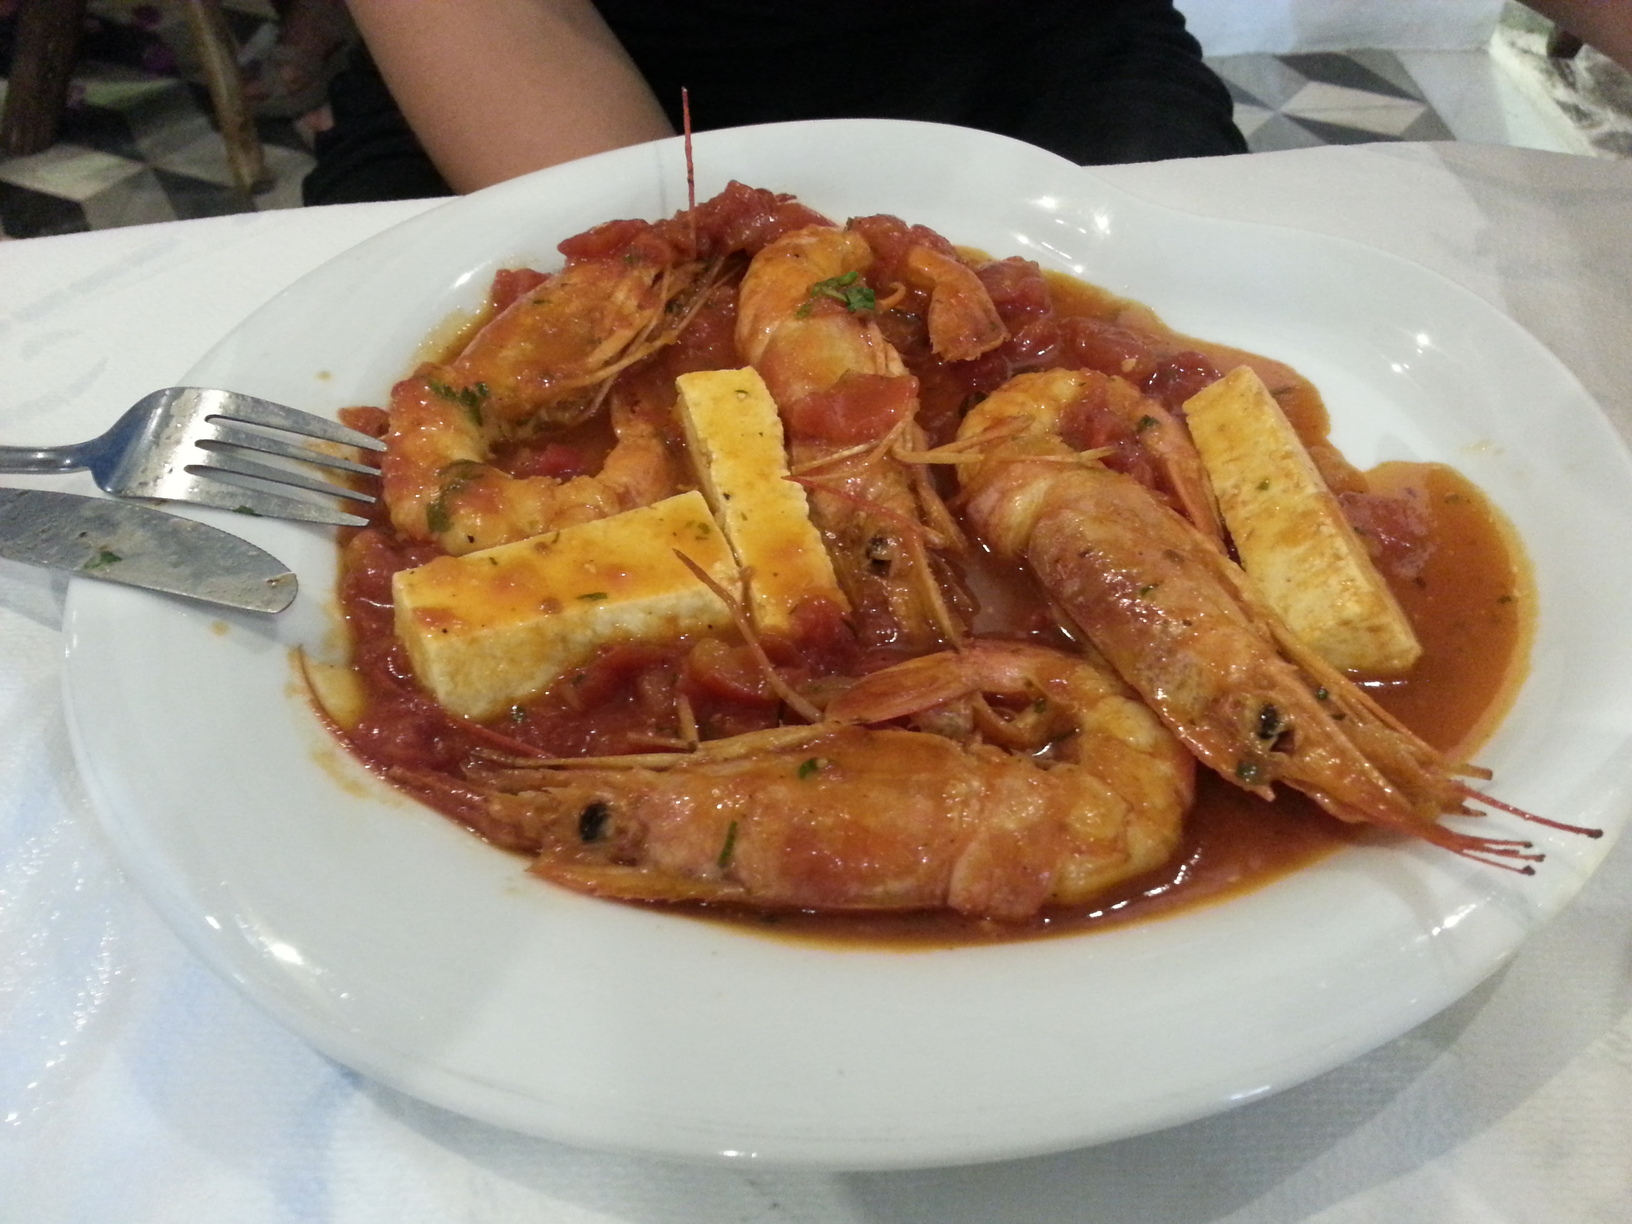
\includegraphics[width=0.32\textwidth]{media/milos_food.jpg}
	\par\textit{Shrimps with cheese from Milos}
\end{center}



%----------------------------------------------------------------------------------------
\NewsItem{Camping with survival?}
% Discuss interesting stories such as Tzia and the almost dry out from water
% Moreover, discuss about Antonis screaming during the night.

%1234567890123456789012345678901234567890123456789012345678901234567890123456789
August is a month where most of the Greeks are resting and replenishing their 
batteries for the new season. 
To this end, we decided to have a camping experience in an island to also chill 
out and to enjoy our time on the beach. 
Our choice was Kea, a rocky and mountaineer island approximately an hour away 
from Lavrio's port.


%1234567890123456789012345678901234567890123456789012345678901234567890123456789
Our team composed from my PhD fellow Antonis Gkortzis (a beard scout boy, 
the man with a solution to every problem, good cold but humour, rum and beer addict), 
Daniela Mikeli (the girl who always smiles, jokes around, and has unlimited energy, 
and looks super cute until she starts drinking beers and watching football games), 
Marios and Maria Zacharia (the sugar couple who recently got a cute pair of twins 
and they are always up for good food and burgers).  
Antonis was our master and commander for the whole camping experience since he was 
following the tradition from his childhood. 


%1234567890123456789012345678901234567890123456789012345678901234567890123456789



%1234567890123456789012345678901234567890123456789012345678901234567890123456789
Time is passing very fast while having fun, but how is it passing when you are not? 
We had to find out in a hard way while we decided to test our survival skills 
with trail walking under the heat of \ang{30} plus.  


%----------------------------------------------------------------------------------------
\NewsItem{Don't say no to raki}
% Discuss about Chania and the driving with Alexandre De Masi in addition the 
% rakia every time that I had to drink







\end{multicols}

% Discuss about Hydra and how Dorine was saying...can we not go back to Athens and stay here?
% Discuss about Aigina with Andreas Tattis
% Discuss about Agkistri with Fisayo.
% Discuss about Leukada with Voijak and the paragliding experience + travelling 8 hours to 
% stay there for a day and a half.

\end{document} 